% flashcards-title: Rounded-value interval band on a centimeter line
% flashcards-desc: A number line from five to seven with a longer labeled mark at each whole centimeter and small steps at tenths between them. A dot sits on the mark at six, and a shaded band along the line surrounds the dot, stretching partway toward five on the left and partway toward seven on the right.
\documentclass[tikz]{standalone}
\usetikzlibrary{arrows.meta,patterns}

\definecolor{qraNavy}{HTML}{17324D}
\definecolor{qraBlue}{HTML}{2B6CB0}
\definecolor{qraGold}{HTML}{B7791F}
\definecolor{qraPale}{HTML}{EAF2F8}
\definecolor{qraGray}{HTML}{5C6773}

\tikzset{
  qra axis/.style={draw=qraNavy, line width=1.2pt},
  qra tick/.style={draw=qraNavy, line width=1pt},
  qra guide/.style={draw=qraGray, densely dashed, line width=0.8pt},
  qra counter/.style={circle, draw=qraNavy, fill=qraPale, line width=0.9pt, minimum size=7mm, inner sep=0pt},
  qra label/.style={font=\sffamily\bfseries, text=qraNavy},
  qra small label/.style={font=\sffamily, text=qraNavy},
}

\begin{document}
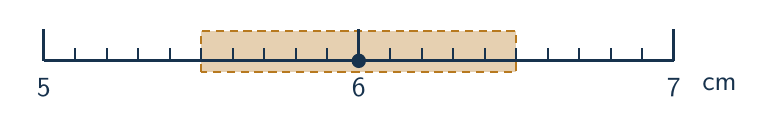
\begin{tikzpicture}[x=4cm,y=1cm]
  % shaded band for values reported as 6 (drawn first so the line stays visible)
  \fill[qraGold!35] (0.5,-0.14) rectangle (1.5,0.38);
  \draw[qra guide, draw=qraGold] (0.5,-0.14) rectangle (1.5,0.38);
  % baseline
  \draw[qra axis] (0,0) -- (2,0);
  % minor ticks at tenths
  \foreach \i in {0,...,20}
    \draw[qra tick, line width=0.6pt] (\i*0.1,0) -- (\i*0.1,0.16);
  % major ticks and labels
  \foreach \x/\l in {0/5,1/6,2/7} {
    \draw[qra tick, line width=1.2pt] (\x,0) -- (\x,0.4);
    \node[qra small label, below] at (\x,-0.1) {\l};
  }
  \node[qra small label, anchor=west] at (2.06,-0.3) {cm};
  % dot at the reported value 6
  \fill[qraNavy] (1,0) circle [radius=2.6pt];
\end{tikzpicture}
\end{document}
